% Title page
\maketitle

\newpage

% Copyright page
\thispagestyle{empty}
\begin{center}
\null
\vfill
\textcopyright 2025 Jee Uhn Kim
\end{center}

\newpage

% Title and abstract page
\thispagestyle{empty}
\begin{center}
{\bf \thesistitle}\\
Jee Uhn Kim\\
Advisor: David Treumann, Ph.D.
\end{center}
\begin{center}
Abstract
\end{center}

In this thesis, we study the moduli space of rank $1$ constructible sheaves on the cylinder $S^1_x \times \R_z$, where the sheaves have vanishing stalks at specified points and singular support contained in a fixed Legendrian link living inside the cocircle bundle of the cylinder. Our focus is on the case where these Legendrian links arise from the cylindrical closures of positive braid words.

In Chapter 2, we introduce a special class of braid words, called \emph{Sibuya braid words}, and show that the corresponding moduli spaces parametrize configurations of points in projective space subject to certain non-degeneracy conditions. We also compute explicit examples of these spaces.

In Chapter 3, we explicitly construct an example from a class of coordinate charts for the moduli space, known as \emph{cluster coordinate charts}.

\frontmatter % Roman page numbering starts here

% Table of contents
\thispagestyle{plain}
\phantomsection
\addcontentsline{toc}{chapter}{Contents}
%\chead{}
\cfoot{\thepage}
\tableofcontents

\newpage

% List of figures
\thispagestyle{plain}
\phantomsection
\addcontentsline{toc}{chapter}{List of Figures}
\cfoot{\thepage}
\listoffigures

\newpage

% Acknowledgments
\thispagestyle{plain}
\phantomsection
\addcontentsline{toc}{chapter}{Acknowledgements}
\cfoot{\thepage}
\vspace*{0.75in}
\begin{center}
{\Large\textbf{Acknowledgments}}
\end{center}
\
\
\noindent
\bigskip

As I complete this thesis, I am deeply grateful to the many individuals who have supported me throughout my academic journey.\\
First and foremost, I would like to express my sincere gratitude to my advisor, Professor David Treumann, whose guidance and support have been crucial in shaping this thesis. What I appreciate most, however, were our enlightening conversations, which shaped not only this thesis but also my approach to problem-solving. I believe this profound influence will continue to guide me in my future career outside of academia.\\
I am thankful to my thesis defence committee members, Professors John Baldwin and Joshua Greene, for their valuable insights and constructive feedback.\\
My time in graduate school has been enriched by the mentorship of many exceptional faculty members. I would like to thank Professors Avner Ash, Ian Biringer, Martin Bridgeman, Dawei Chen, Qile Chen , Solomon Friedberg, Benjamin Howard, Xin Jin, and Robert Meyerhoff for their teachings and encouraging my academic growth.\\
The time I spent at Boston College was one of the happiest periods of my life. Thank you Ethan Farber, Yin Nam Dalton Fung, Stella Sue Gastineau, Iulia Gheorghita, Hao Li, Siddharth Mahendraker, Martha McAlister-Raeburn, Eric Moss, Braeden Reinoso, Fraser Malcom Watt Binns, Yifan Wu, and Cemre Yavuz for sharing beautiful memories.\\
I would also like to thank the professors from my undergraduate years who ignited my interest in math: Professors Sung Rak Choi, Haseo Ki, Joonil Kim, and June Bok Lee.\\
I send my deepest gratitude to friends who supported me away from home: Choonwon B. Kim, Heejong Lee, Seungsu Lee, Jinhan Park, Jonghyeon Park, Donggeun Ryou, Michael Schreiber, and Patrick Yoon. This journey would have been a lot more difficult without your help.\\
I am grateful to my cousins in America, Charles, Henry, and Mary Noh, and in Korea, Jong Hwa Park and Ji Eun Lee, for making me feel at home regardless of where I was.\\
To my grandparents, Ja Heon Kim, Kye Sung Chung, Young Ok Park and Jung Seb Yoon, thank you for your wisdom, love, and the values you taught me.\\
My heartfelt thanks to my family: Sung Ha Kim, Woon Mee Park, Hee Uhn Kim, and Haru Kim. Your unconditional love, patience, and support have been my constant source of strength and motivation.\\
Finally, Chaewon, thank you for believing in me and staying by my side during my most difficult times. Just as we've shared challenging moments together, I hope we can also share many good times together in the future.\\
Although this thesis bears my name, I believe it to be a product of the collective support from all these individuals. Any flaws, however, remain entirely my own.


\newpage

\mainmatter % Standard page numbering starts here

%%%%%%%%%%%%%%%%%%%%%%%%%%%%%%%%%%%%%%%%%%%%%%%%%%%%%%%%%%%%%%%%%%%%%%%%%%%%%%%%%%%%%%%%
%%%%%%%%%%%%%%%%%%%%%%%%%%%%%%%%%%%%%%%%%%%%%%%%%%%%%%%%%%%%%%%%%%%%%%%%%%%%%%%%%%%%%%%%

\chapter{Introduction}\label{chapter_introduction}

\section{Background and context}\label{sec_background_and_context}

\subsection*{Contact Geometry}
First, we review basics of contact geometry, see \cite{etnyre2005legendrian}\cite{geiges2008introduction} for details. A contact structure on a $(2n-1)$-dimensional manifold $X$ is a maximally nonintegrable distribution of $(2n-2)$-planes. A contact structure defined globally as a kernel for a chosen $1$-form $\alpha$ is said to be co-oriented and $\alpha$ is said to be its co-orientation. An $(n-1)$-dimensional submanifold $\Lambda \subset X$ is said to be Legendrian if its tangent bundle is contained in the contact hyperplanes. Now let's look at several examples of contact manifolds.
\begin{enumerate}[label = (\arabic*)]
\item the contagent bundle $T^*M$ of a manifold $M$ carries a canonical $1$-form which is in local coordinates $(q_i,p_i)$, $\theta := \underset{i}{\sum} p_i dq_i$. This form is invariant under dialation in cotangent directions, therefore, $\theta$ descends to a well-defined $1$-form(unique up to positive scalar function) on the cosphere bundle $T^\infty M := (T^*M - 0_M)/\R_+$ where $0_M$ is the zero section and $\R_+$-action is the dialation action along cotangent directions. Therefore, $T^\infty M$ is equipped with a natural contact structure.

\item $\R^3_{x,y,z}$ with the global $1$-form $\alpha = dz - ydx$ defines a co-oriented contact structure. We can embed $\R^3_{x,y,z}$ in $T^{\infty,-}\R^2_{x,z}$ as an open contact submanifold as follows:
\begin{align*}
\R^3_{x,y,z} &\rightarrow \R^2_{x,z} \times S^1 \\
(x,y,z) & \mapsto (x,z;y,-1)
\end{align*}
The image is the contact submanifold $T^{\infty,-}\R^2_{x,z}$ of "downward" covectors.

\item Note that construction $(2)$ is invariant under translation $x \mapsto x+1$. Let $S^1_x := \R_x / \Z$, then standard $1$-form $dz - ydx$ descends to $S^1_x \times \R_{y,z}$ and it embeds as the contact submanifold $T^{\infty, -}(S^1_x \times \R_z)$ in $T^\infty(S^1_x \times \R_z)\cong S^1_x \times \R_z \times S^1_y$. The``cocircle bundle" in the title of the thesis refers to $T^\infty (S^1_x \times \R_z)$.
\end{enumerate}

\subsection*{Front Projection}
Now let's restrict our attention to the case when the base manifold $M$ is either $\R^2_{x,z}$ or $S^1_x \times \R_z$. We call the map $\pi : T^\infty M \rightarrow M$ the "front projection" and $\pi(\Lambda)$ the ``front diagram".
\begin{itemize}
\item when $M = \R^2_{x,z}$, $\pi : \R^3_{x,y,z} \subset T^\infty \R^2_{x,z} \rightarrow \R^2_{x,z}$ is the projection onto $x,z$ coordinates. We call $\R^2_{x,z}$ a front plane.

\item similarly, when $M = S^1_x \times \R_{z}$, $\pi : S^1_x \times \R^2_{y,z} \subset T^\infty (S^1_x \times \R_{z}) \rightarrow S^1_x \times \R_{z}$ is the projection onto $x,z$ coordinates. We call $S^1_x \times \R_{z}$ a front cylinder.
\end{itemize}
A Legendrian $\Lambda \subset T^{\infty}M$ at immersed points of $\pi(\Lambda)$can be recovered from $\pi(\Lambda)$ because $\Lambda$ vanishes on the contact form $dz-ydx$, we have $y = \frac{dz}{dx}$ as long as it is in general position. Under Hamiltonian isotopy, $\Lambda$ can be put in general position, i.e.
\begin{itemize}
\item $\pi|_\Lambda$ is locally injective.

\item there are only finitely many points on $M$ at which $\pi(\Lambda)$ is not an embedded submanifold. These are either
\begin{itemize}
\item cusps where $\pi|_{\Lambda}$ is injective and $\frac{dz}{dx}$ has a well-defined limit of $0$.

\item crossing where $\pi(\Lambda)$ is locally a transverse intersection of two smooth curves.
\end{itemize}
\end{itemize}
In this paper, we only allow $\pi(\Lambda)$ to have crossings. We won't consider $\pi(\Lambda)$ with cusps. There are no interesting examples in $\R^3_{x,y,z}$ but there are many interesting ones in the cocircle bundle of a cylinder.
Suppose we have a smooth parametrized curve $\Phi$ in $M$
\begin{itemize}
\item which is an immersion

\item which has finitely many self-intersections and they are transverse.
\end{itemize}
and a choice of preferred side, i.e. a co-orientation, diagramatically described using hairs normal to the $\Phi$ pointing the preferred direction. We say that the region on the preferred side lies beneath the  the arc and the region on the other side lies above the arc. We can lift it to a Legendrian in $T^{\infty}M$. Therefore, the Legendrian in $T^{\infty}M$ amounts to the datum of the co-oriented front diagram.

\subsection*{Constructible sheaves}
Let $M$ be a manifold and $\mathcal{S}$ Whitney a stratification of $M$. A sheaf of $\C$-vector space $\mathscr{F}$ on $M$ is $\mathcal{S}$-constructible if the restriction of $\mathscr{F}$ to each stratum of $s\in \mathcal{S}$, $\mathscr{F}|_s$, is a locally constant sheaf. $\mathscr{F}$ is called constructible if there exists a Whitney stratification $\mathcal{S}$ such that $\mathscr{F}$ is $\mathcal{S}$-constructible.
$Sh^\bullet_{naive}(M;\C)$ denotes the triangulated dg category whose objects are cochain complexes of sheaves of $\C$-vector spaces of bounded cohomology whose cohomology sheaves are constructible sheaves. If we localize $Sh^\bullet_{naive}(M;\C)$ with respect to acyclic complexes, in the sense of \cite{drinfeld2004dg}, we get $Sh^\bullet(M;\C)$. We denote $Sh^\bullet_{\mathcal{S}}(M;\C)$ the full subcategory of $Sh^\bullet (M;\C)$ of complexes whose cohomology sheaves are constructible with respect to $\mathcal{S}$. From now on we will call objects of $Sh^\bullet(M;\C)$ simply as sheaves.\\

\subsection*{Singular Support}
To each $\mathscr{F}\in Sh^\bullet (M;\C)$, we assign a closed conical subset $SS(\mathscr{F})\subset T^*M$, called the singular support of $\mathscr{F}$ following \cite{goresky1983stratified}\cite{schurmann2012topology}\cite{shende2017legendrian}. For more general treatment, see \cite{kashiwara2013sheaves}. Fix a Riemannian metric on $M$ and choose an $\epsilon$-ball $B_\epsilon(x)$ around a point $x\in M$. The following constructions are independent of the choice of metrics. Let $\mathscr{F}$ be an $\mathcal{S}$-constructible sheaf on $M$. Fix a point $x\in M$ and a smooth function $f$ on $B_\epsilon(x)$. For $\epsilon,\delta >0$, we define the local Morse group to be
\[
Mo_{x,f,\epsilon,\delta}(\mathscr{F}) := H^*(B_\epsilon(x)\cap f^{-1}((-\infty,f(x)+\delta)),B_\epsilon(x)\cap f^{-1}((-\infty,f(x)-\delta));\mathscr{F})
\]
For $\epsilon' < \epsilon$ and $\delta' < \delta$, there is a canonical restriction map
\[
Mo_{x,f,\epsilon,\delta}(\mathscr{F})\rightarrow Mo_{x,f,\epsilon',\delta'}(\mathscr{F})
\]
The above restriction is an isomorphism if $\epsilon$ and $\delta$ are sufficiently small and $f$ is stratified Morse at $x$. This allows us to define $Mo_{x,f}(\mathscr{F})$ for $f$ suitably generic with respect to $\mathcal{S}$\cite[Prop.~7.5.3]{kashiwara2013sheaves}. In fact, $Mo_{x,f} (\mathscr{F})$ depends only on the Hessian of $f$ at $x$.
Let $\mathscr{F}\in Sh^\bullet (M;\C)$, then $(x,\xi)\in T^*M$ is characteristic with respect to $\mathscr{F}$ if for some stratified Morse function $f$ with $df_x = \xi$, the local Morse group $Mo_{x,f}(\mathscr{F})$ is nonzero. Then we define the singular support of $\mathscr{F}$ to be the closure of the set of characteristic covectors for $\mathscr{F}$ in $T^*M$. Singular support is a conic Lagrangian i.e. stable under $\R_+$-dialation along contangent fibers.\\
Fix a conic Lagrangian $L\subset T^*M$, then we define $Sh^\bullet_L(M;\C)$ to be the full subcategory of $Sh^\bullet_L(M;\C)$ whose objects are sheaves singular supported in $L$. If $\Lambda\subset T^\infty M$ is a Legendrian, then we define $Sh^\bullet_\Lambda(M;\C) := Sh^\bullet_{\R_+ \Lambda \cup 0_M}(M;\C)$ where $0_M \subset T^*M$ is the zero section.

\subsection*{Combinatorial Model of $Sh^\bullet_\Lambda(M;\C)$}
The first necessary condition for $\mathscr{F}\in Sh^\bullet(M;\C)$ to belong to $Sh^\bullet_L(M;\C)$ is that $\mathscr{F}$ is constructible with respect to the stratification on $M$ induced by the front projection of $\Lambda$. That is the Whitney stratification whose zero dimensional strata are crossings, one dimensional strata are the arcs of $\pi(\Lambda)$ between crossings and two dimensional strata are the connected components of the complement of $\pi(\Lambda)$ in $M$.

\begin{definition}
Given a stratification $\mathcal{S}$, the star of a stratum $s\in \mathcal{S}$ is the union of strata that contain $s$ in their closure. We view $\mathcal{S}$ as a poset category $s\leq t$ if and only if $s \subset \overline{t}$. We call the map from $s$ to $t$ as a generization map. We say $\mathcal{S}$ is a regular cell complex if every stratum is contractible and moreover the star of each stratum is contractible.
\end{definition}

\begin{definition}
We define $Fun^\bullet_{naive}(\mathcal{S},\C)$ to be the dg category of functors from $\mathcal{S}$ to the category whose objects are cochain complexes of $\C$-vector spaces and whose maps are cochain maps. 
We define $Fun^\bullet(\mathcal{S}, \C)$ the dg quotient \cite{drinfeld2004dg} of $Fun^\bullet_{naive}(\mathcal{S},\C)$ by the thick subcategory of functors taking values in acyclic complexes.
\end{definition}

\begin{proposition}\label{KS}
\cite{kashiwara1984riemann}, \cite{shepard1985cellular}, \cite[Lemma~2.3.2]{nadler2009microlocal}.Let $\mathcal{S}$ be a Whitney stratification of $M$. Consider the functor 
\begin{align*}
&\Gamma_\mathcal{S} : Sh^\bullet_\mathcal{S}(M;\C) \rightarrow Fun^\bullet(\mathcal{S},\C)\\
&\mathscr{F} \mapsto [s\mapsto \Gamma(star(s);\mathscr{F})]
\end{align*}
If $\mathcal{S}$ is a regular cell complex, then $\Gamma_\mathcal{S}$ is a quasi-equivalence.
\end{proposition}
However, the stratification induced by the front diagram is not necessarily a regular cell complex. Therefore, we choose an $\mathcal{S}$ that refines of the stratification induced by $\pi(\Lambda)$. In figures, we draw the new line segments in squiggly lines. \\
The restriction of $\Gamma_\mathcal{S}$ to $Sh^\bullet_\Lambda(M;\C)$ is quasi-fully faithful. We will describe the essential image of $Sh^\bullet_\Lambda(M;\C)$ under $\Gamma_\mathcal{S}$.

\begin{definition}
Let $\mathcal{S}$ be a regular cell complex refining the stratification induced by the front diagram. we define $Fun^\bullet_\Lambda(\mathcal{S},\C)$ to be the full subcategory of $Fun^\bullet(\mathcal{S},\C)$ whose objects satisfy the following properties.
\begin{itemize}
\item every map from a zero dimensional stratum in $\mathcal{S}$ which is not a crossing is sent to quasi-isomorphism.

\item every map from a one dimensional stratum which is not contained in an arc is sent to quasi-isomorphism.

\item for each crossing $c\in \mathcal{S}$, Let $N$, $E$, $S$, $W$ be the north, east, south, and west regions adjoining $c$, and let $nw$, $ne$, $sw$, $se$ be the arcs separating them.
\begin{figure}[H] 
    \centering
    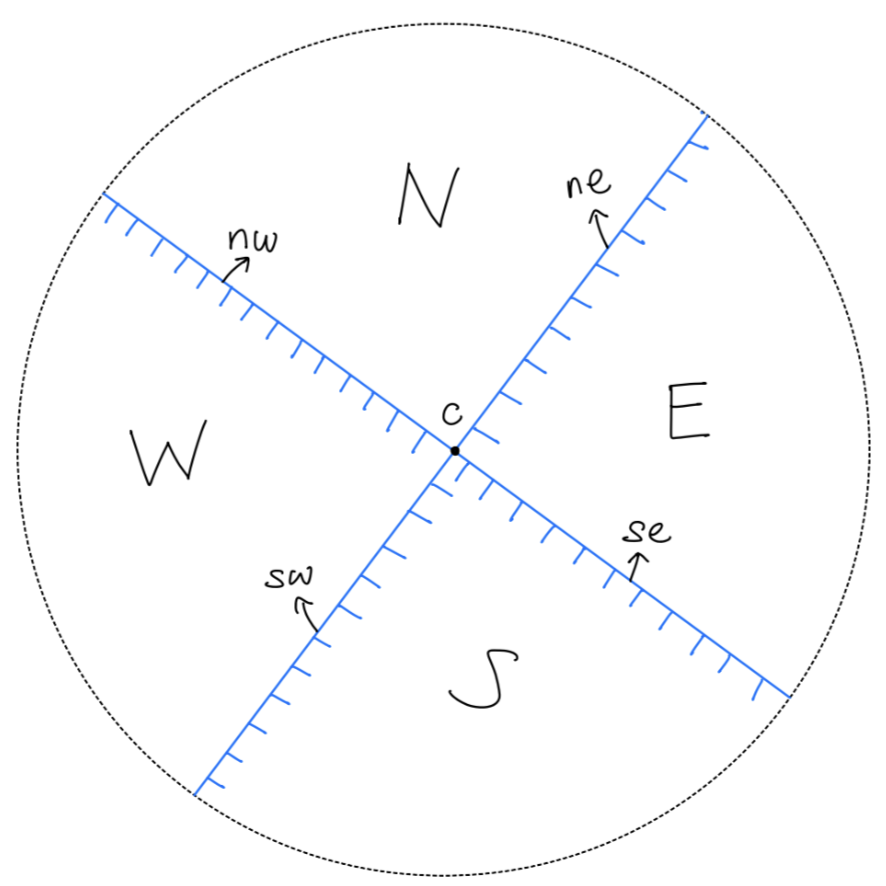
\includegraphics[scale = 0.55]{diagrams/intro/1.png}
    \caption{}
    \label{fig:your-label}
\end{figure}
Then the following maps are sent to quasi-isomorphisms.
\begin{itemize}
\item maps between $c$, $sw$, $se$, and $S$.
\item a map from $nw$ to $W$.
\item a map from $ne$ to $E$.
\end{itemize}

\item for each crossing $c\in \mathcal{S}$, we restrict the poset structure to the strata containing $c$ in its closure, we get
\[
\begin{tikzcd}
& & N & &\\
& nw\arrow[ur]\arrow[dl] & & ne\arrow[ul]\arrow[dr] &  \\
W& & c\arrow[uu]\arrow[dd]\arrow[ll]\arrow[rr]\arrow[ul]\arrow[ur]\arrow[dl]\arrow[dr] & & E \\
& sw\arrow[ul]\arrow[dr] & & se\arrow[ur]\arrow[dl] &  \\
& & S & &\\
\end{tikzcd}
\]
Then all triangles in the diagram should commute and the total complex of the following bicomplex 
\[
F(c)\rightarrow F(nw)\oplus F(ne) \rightarrow F(N)
\]
should be acyclic.
\end{itemize}
\end{definition}
A standard argument shows that the essential image of  $Sh^\bullet_\Lambda(M,\C)$ under $\Gamma_\mathcal{S}$ is $Fun^\bullet_\Lambda(\mathcal{S},\C)$\cite{shende2017legendrian}.

\subsection*{Legible Objects}
Let $M$ be a front surface, $\Phi$ a front diagram, $\Lambda \subset T^{\infty}M$ the associated Legendrian knot, and $\mathcal{S}$ a refinement of the stratification induced by $\Phi$ by adding squiggly lines. In this section, we define a ``legible quiver" and a ``squiggly legible diagram" to get a better handle on $Fun^\bullet_\Lambda(M;\C)$.\\
Suppose we impose an auxiliary co-orientation on the squiggly lines as well, then this induces a quiver $Q$ 
\begin{definition}
Suppose we have a regular cell complex $\mathcal{S}$ that refines the stratification induced by $\Phi$ with auxiliary co-orientations on the added squiggly lines segments, then we define the associated quiver $Q$ where
\begin{itemize}
\item the vertices of $Q$ are $2$ dimensional strata
\item the arrows of $Q$ are $1$ dimensional strata where the sources and the targets are regions below and above the strata.
\end{itemize}
For a stratum $s\in \mathcal{S}$, we define $Q_s$ to be the full sub-quiver of $Q$ whose vertices are the regions incident with $s$.
\end{definition}

\begin{definition}
We say that the quiver associated to $\mathcal{S}$ is \emph{legible} if 
for every point stratum $p\in \mathcal{S}$, the sub-quiver $Q_p$ is a poset with the smallest element.
\end{definition}

\begin{definition}
A squiggly legible diagram on $\mathcal{S}$ is the representation $F^\bullet$ of the quiver $Q$ associated to $\mathcal{S}$ valued in the cochain complex of $\C$-vector spaces subject to the condition that
\begin{itemize}
\item the maps corresponding to squiggly lines are quasi-isomorphisms.

\item for fixed a source and a target vertices $s$ and $t$, suppose we have to distinct paths in $Q$(a sequence of arrows) from $s$ to $t$, say $(a_1,a_2,\cdots,a_k)$ and $(a'_1,a'_2,\cdots,a'_l)$, then $F^\bullet(a_k)\circ \cdots \circ F^\bullet(a_1) = F^\bullet(a'_l)\circ \cdots \circ F^\bullet(a'_1)$ i.e. the composition of cochain maps are path independent.

\item at each crossing, we have surrounding region $N,S,W,E$
\begin{figure}[H] 
    \centering
    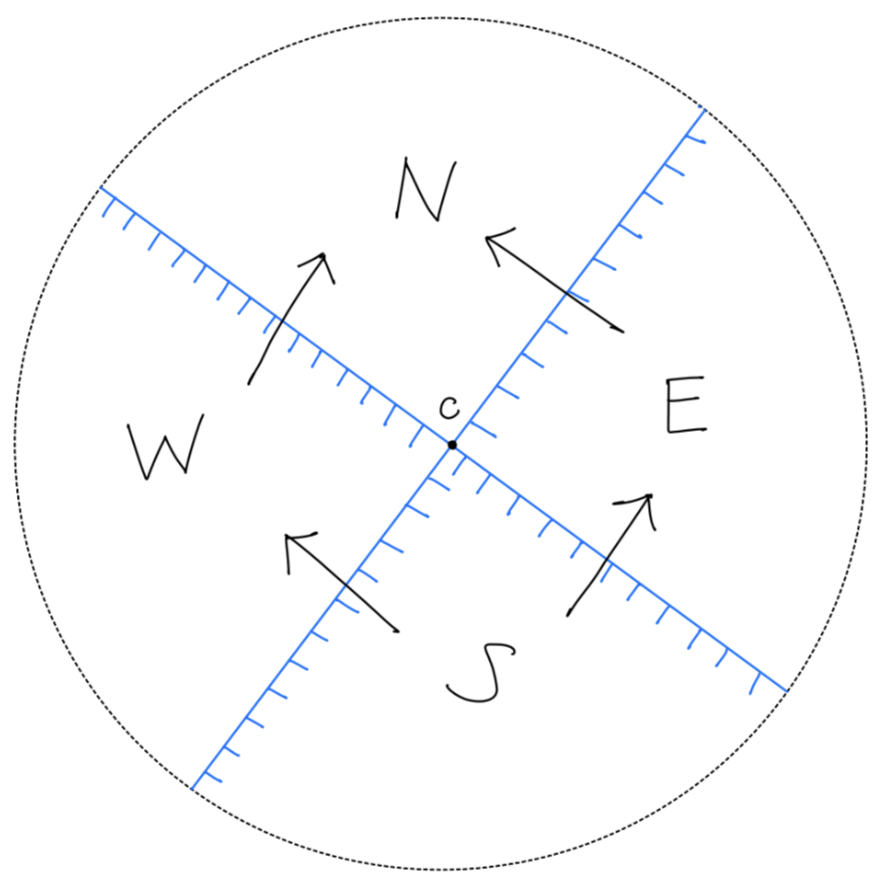
\includegraphics[scale = 0.55]{diagrams/intro/2.png}
    \caption{}
    \label{fig:your-label}
\end{figure}
then the total complex of 
\[
F^\bullet(S) \rightarrow F^\bullet(W)\oplus F^\bullet(E) \rightarrow F^\bullet(N)
\]
is acyclic.
\end{itemize}
\end{definition}
Suppose we have $\mathcal{S}$ a refinement of the stratification induced by $\Phi$ and a squiggly legible diagram $F^\bullet$, then we can make an object $\overline{F}^\bullet \in Fun^\bullet_\Lambda(\mathcal{S},\C)$ out of it in the following way.
\begin{definition}
$\rho : \mathcal{S} \rightarrow \{R\in \mathcal{S} \mid dim_\R(R) =2\}$ is a function that assigns $s\in \mathcal{S}$ to the smallest element in $\{R\in Vert(Q) \mid s \subset \overline{R}\}$.
\end{definition}

\begin{definition}
Suppose $F^\bullet$ is a squiggly legible diagram on $\mathcal{S}$, then we define $\overline{F}^\bullet \in Fun^\bullet _\Lambda (\mathcal{S},\C)$ where 
\begin{itemize}
\item for $s\in \mathcal{S}$, $\overline{F}^\bullet(s) := F^\bullet(\rho(s))$

\item for $s_1,s_2 \in \mathcal{S}$ such that $s_2 \subset star(s_1)$, $\overline{F}^\bullet (s_1 \rightarrow s_2) := F^\bullet(a_k)\circ \cdots F^\bullet(a_1)$ where $(a_1,a_2,\cdots,a_k)$ is a path from $\rho(s_1)$ to $\rho(s_2)$ in the quiver associated to $\mathcal{S}$. This is well-defined because the composition of cochain maps are path independent by the definition of squiggly legible diagram and the existence of a path from $\rho(s_1)$ to $\rho(s_2)$ is guaranteed by the fact that $Q_{s_2}$ is a subquiver of $Q_{s_1}$ and $\rho(s_2),\rho(s_1)$ are the smallest elements from each of them.
\end{itemize}
\end{definition}
In this paper, we only consider $\Phi$, $\Lambda$, and $\mathcal{S}$ that objects of $Fun^\bullet(\mathcal{S},\C)$ arises from squiggly legible diagrams.A variant of \cite[Prop~3.22.]{shende2017legendrian} shows that every objects of $Sh^\bullet_\Lambda(M;\C)$ is quasi-isomorphic to a squiggly legible diagram.

\subsection*{Microlocal Monodromy and Rank $1$ Objects}
In this section, we review the notion of microlocal monodromy of sheaves following\cite[Section~5.1]{shende2017legendrian}. For more general treatment, see \cite[Ch.~\MakeUppercase{\Rn{4}}]{kashiwara2013sheaves}. Supppose on $M$ we have a front diagram $\Phi$ and a stratification $\mathcal{S}$ that refines the one induced by $\Phi$ by adding squiggly line segments. Suppose we are given a sheaf $F^\bullet$ in terms of squiggly legible diagram, we define the associated sheaf on $\Lambda$, called microlocal monodromy denoted $\mu mon (F^\bullet)$, by assigning cochain complexes of $\C$-vector spaces for each one dimensional stratum contained in $\Phi$ and cochain maps between them for each point stratum contained in $\Phi$ as follows:
\begin{itemize}
\item if $s$ is a one dimensional stratum contained in $\Phi$, $\mu mon (F^\bullet)(s):=Cone(F^\bullet(s))$

\item if $p$ is a point stratum in $\Phi$, then $p$ is either a crossing or the endpoint of a squiggly line. We define the cochain map for each case as follows:
\begin{itemize}
\item when $p$ is a crossing, locally near $p$ the diagram looks like
\begin{figure}[H] 
    \centering
    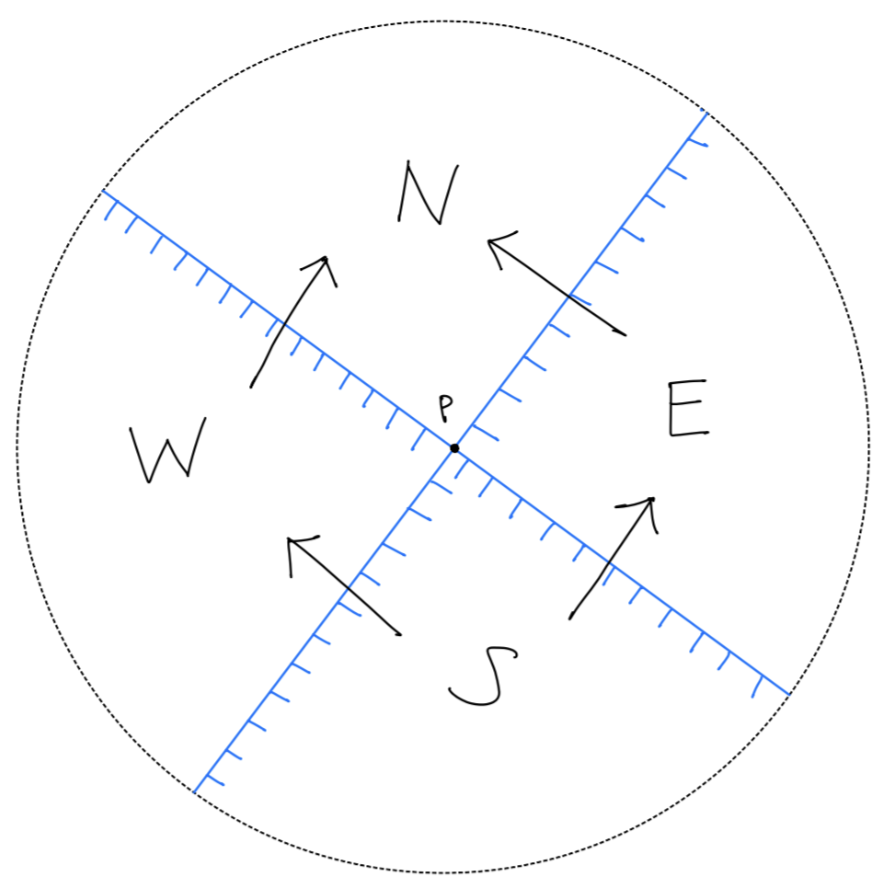
\includegraphics[scale = 0.55]{diagrams/intro/3.png}
    \caption{}
    \label{fig:your-label}
\end{figure}
then $p$ induces maps
\begin{align*}
& Cone(S\rightarrow W) \rightarrow Cone(E\rightarrow W)\\
& Cone(S\rightarrow E) \rightarrow Cone(W\rightarrow N)\\
\end{align*}

\item when $p$ is the endpoint of a squiggly line segment, locally near $p$ the diagram looks like one of the following diagrams 
\begin{figure}[H] 
    \centering
    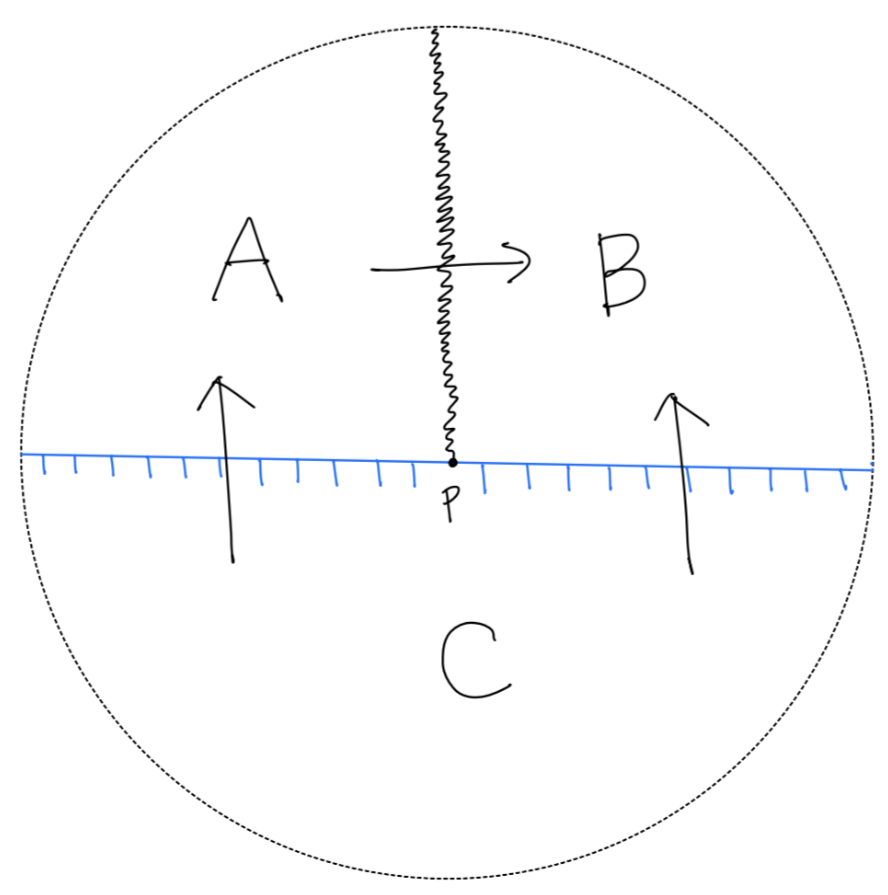
\includegraphics[scale = 0.55]{diagrams/intro/4.png}
    \caption{}
    \label{fig:your-label}
\end{figure}
\begin{figure}[H] 
    \centering
    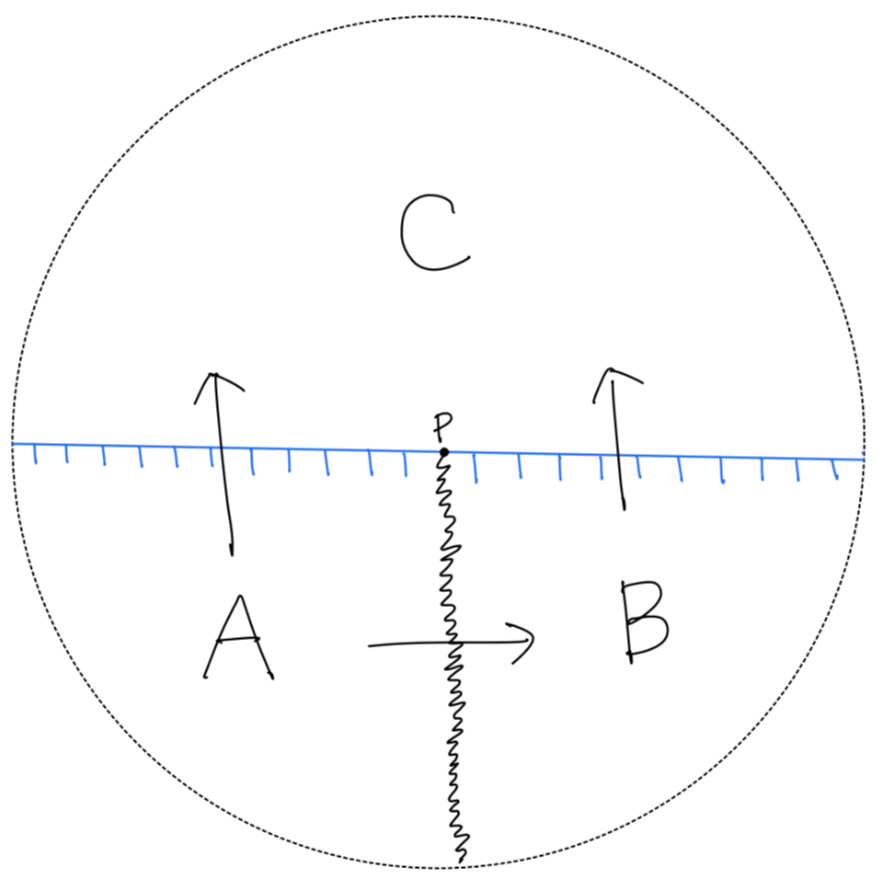
\includegraphics[scale = 0.55]{diagrams/intro/5.png}
    \caption{}
    \label{fig:your-label}
\end{figure}
\begin{figure}[H] 
    \centering
    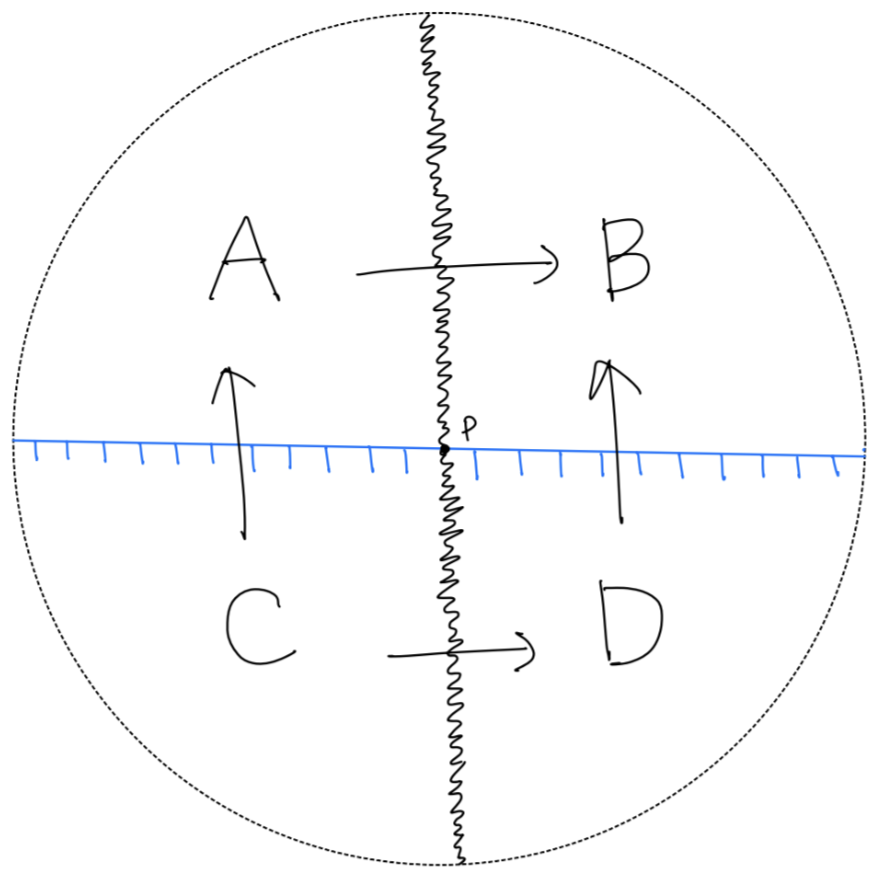
\includegraphics[scale = 0.55]{diagrams/intro/6.png}
    \caption{}
    \label{fig:your-label}
\end{figure}
, then we have a map
\begin{align*}
& Cone(C\rightarrow A) \rightarrow Cone(C\rightarrow B)\\
& Cone(A\rightarrow C) \rightarrow Cone(B\rightarrow C)\\
& Cone(C\rightarrow A) \rightarrow Cone(D\rightarrow B)\\
\end{align*}
respectively.
\end{itemize}
\end{itemize}
The maps between cones are quasi-isomorphisms because of the crossing condition and the fact that the map corresponding to squiggly lines are quasi-isomorphism.

\begin{definition}
$F^\bullet$ is called \emph{rank $n$ object} if $\mu mon (F^\bullet)$ is a rank $n$ local system concentrated in degree $0$ on $\Lambda$.
\end{definition}

\begin{definition}
The full subcategory of $Sh^\bullet_\Lambda(M;\C)$ containing rank $n$ objects is denoted $\mathcal{C}_n(M,\Lambda;\C)$ and the moduli stack classifying such objects $\mathcal{M}_n(M,\Lambda;\C)$. Additionally, let $\{\sigma_1,\cdots,\sigma_k\}$ be points in $M$ that are contained in one of the regions separated by $\Phi$. Then we define $\mathcal{C}_n(M,\Lambda, \{\sigma_1,\cdots,\sigma_k\};\C)$ to be the full subcategory of sheaves with vanishing stalks at $\{\sigma_1,\cdots,\sigma_k\}$, $\mathcal{M}(M,\Lambda, \{\sigma_1,\cdots,\sigma_k\};\C)$ the moduli space classifying such objects.
\end{definition}

\subsection*{Moduli Spaces associated to Positive Braids}
In this section, we define the moduli spaces associated to positive braids following\cite[Section~3]{shende2019cluster}. For background we refer to the survey \cite{toen2014derived} and the foundational works \cite{lurie2004derived} \cite{toen2009higher} \cite{toen2004hag} \cite{toen2005homotopical} \cite{toen2008homotopical}. Suppose we have a positive braid word $\omega$ of $n$ strands(i.e. a word freely generated by $s_1,\cdots,s_{n-1}$), Then we can think of its cylindrical closure in $S^1_\theta \times (0,1)_r = (\R_\theta /\Z) \times (0,1)_r$. In this paper, we consider two kinds of moduli spaces associated to the braid which are the main objects of study in Chapter2 and Chapter3 respectively.
\begin{enumerate}[label = (\arabic*)]
\item First, we embedd the cylinder containing cylindrical closure of $\omega$ in $M = S^1_x \times \R_z$ via $(\theta, r)\mapsto (\theta, r-1)$. We can think of the cylindrical closure of $\omega$ in $S^1_x \times \R_z$ co-oriented downward($z<0$) to be the front projection of a Legendrian knot $\Lambda_\omega$ living in $T^{\infty}M$. Let $\sigma_{z\ll 0}$ be a point in the non-compact region where $z\ll 0$. In Chapter2, we consider the moduli space $\mathcal{M}_1(S^1_x\times \R_z, \Lambda_\omega,\{\sigma_{z\ll 0}\};\C)$.

\item Next, we embed the cylinder containing the cylindrical closure of $\omega$ in $M = S^1_x \times \R_z$ via $(\theta,r) \mapsto (\theta,1-r)$ and embed the cylinder containing the cylindrical closure of the trivial braid $\omega_\emptyset$ via $(\theta,r)\mapsto (\theta,r-1)$. We get an embedding of the cylindrical closure of $\omega \coprod \omega_\emptyset$ in $S^1_x \times \R_z$ where the embedding of the cylindrical closure of $\omega$ is co-oriented upward and the embedding of the cylindrical closure of $\omega_\emptyset$ is co-oriented downward. We will call the embedding the separated diagram of $\omega$ and $\omega_\emptyset$ which we consider as the front projection of a Legendrian link $\Lambda_{\infty} \coprod \Lambda_{0} \subset T^{\infty}M$. Let $\sigma_{z\ll 0},\sigma_{z\gg 0}$ be points in the non-compact regions where $z\ll 0$ and $z\gg 0$. In Chapter3, we consider the moduli space $\mathcal{M}_1(S^1_x\times \R_z, \Lambda_\omega \coprod \Lambda_{\omega_\emptyset},\{\sigma_{z\ll 0}, \sigma_{z\gg 0}\};\C)$.
\end{enumerate}

\subsection*{Legendrian Isotopy and Sheaf Cobordism}
Invariance of the category $\mathcal{C}_1(M,\Lambda, \{\sigma_1,\cdots,\sigma_k\};\C)$ under Legendrian isotopy follows from the main theorem of \cite{guillermou2012sheaf}.
\begin{theorem}\label{GKS}
\cite{guillermou2012sheaf}. Suppose $\Lambda_0 \subset T^{\infty}M$ is a Legendrian and $\Lambda_\bullet \subset T^{\infty} \times [0,1]$ a Legendrian isotopy where $\Lambda_\bullet|_{T^{\infty} \times \{0\}}$ is equal to $\Lambda_0$ under the natural identification $T^{\infty} \times \{0\} \cong T^{\infty}$, then the restriction functor 
\[
Sh^\bullet_{\Lambda_\bullet}(M\times [0,1];\C) \rightarrow Sh^\bullet_{\Lambda_0}(M;\C)
\]
is a quasi-equivalence. Furthermore, this quasi-equivalence preserves rank $n$ objects.
\end{theorem}

\begin{definition}
Suppose we have a Legendrian isotopy $\Lambda_\bullet\subset T^{\infty} \times [0,1]$ from $\Lambda_0 = \Lambda_\bullet|_{T^{\infty} \times \{0\}}$ to $\Lambda_1 = \Lambda_\bullet|_{T^{\infty} \times \{1\}}$ and a sheaf $\mathscr{F}_\bullet \in Sh^\bullet_{\Lambda_\bullet}(M\times [0,1];\C)$ that restricts to $\mathscr{F}_0$ and $\mathscr{F}_1$ at $M\times\{0\}$ and $M\times\{1\}$, then we say $\mathscr{F}_\bullet$ is a \emph{sheaf cobordism} from $\mathscr{F}_0$ to $\mathscr{F}_1$.
\end{definition}

\begin{definition}
Suppose $\Lambda_0,\Lambda_1 \subset T^{\infty}M$ are Legendrian links and there is a Legendrian isotopy $\Lambda_\bullet \subset T^{\infty,-}M \times [0,1]$ where $\Lambda_\bullet|_{T^{\infty,-}\times \{0\}}$ is equal to $\Lambda_0$ under the natural identification $T^{\infty,-}\times \{0\} \cong T^{\infty,-}$ and $\Lambda_\bullet|_{T^{\infty,-}\times \{1\}}$ is equal to $\Lambda_0$ under the natural identification $T^{\infty,-}\times \{1\} \cong T^{\infty,-}$, then we have quasi- equivalence 
\[
Sh^\bullet_{\Lambda_0}(M;\C) \xrightarrow{\sim} Sh^\bullet_{\Lambda_1}(M;\C)
\]
from the following correspondence
\[
Sh^\bullet_{\Lambda_0}(M;\C) \xleftarrow{\sim} Sh^\bullet_{\Lambda_\bullet}(M\times [0,1];\C) \xrightarrow{\sim} Sh^\bullet_{\Lambda_1}(M;\C)
\]
Furthermore, this quasi-equivalence restricts to 
\[
\mathcal{C}_n(M,\Lambda_0;\C) \xrightarrow{\sim} \mathcal{C}(M,\Lambda_1;\C)
\]
When we have points $\{\sigma_1,\cdots,\sigma_k\}\subset M$ that are disjoint from the front projections of the Legendrian isotopy $\Lambda_\bullet$, we can further restrict the quasi-equivalence to
\[
\mathcal{C}_n(M,\Lambda_0,\{\sigma_1,\cdots,\sigma_k\};\C) \xrightarrow{\sim} \mathcal{C}_n(M,\Lambda_1,\{\sigma_1,\cdots,\sigma_k\};\C)
\]
\end{definition}

\subsection*{Alternating Legendrians}
\begin{definition}
Let $M$ be a surface and $\Lambda \subset T^{\infty}M$ a Legendrian link. An \emph{alternating coloring} for $\Lambda$ is the datum of, for each region in the complement of the front diagram, a label of black, white, or null, subject to the following conditions
\begin{itemize}
\item the boundary of a black region is co-oriented inward.
\item the boundary of a white region is co-oriented outward.
\item the boundary of the null region have both inward and outward co-orientations.
\item no black region shares a one dimensional border with white region and no null region shares a one dimensional border with another null region.
\end{itemize}
An \emph{alternating Legendrian} is a Legendrian equipped with an alternating coloring and their front projection is called an \emph{alternating strand diagram}. The \emph{bipartite graph} of the alternating Legendrian is the graph whose vertices are black and white regions. Edges are connected if their closure intersect and are of distinct color.
\end{definition}
Let $\hat{M}$ denote the real blow up of $M$ at the crossings of the front projection of $\Lambda$. The blow down map $\hat{M}\rightarrow M$ is a diffeomorphism away from the crossing and the fiber above a crossing is the $\R \mathbb{P}^1$ of lines tangent to the crossing. We define $W\subset M$($B\subset M$ resp.) the union of the interiors of the white(black resp.) regions of the complement of the front projection.

\begin{definition}
$\overline{L}$ denote the closure of the preimage of $W\cup B$ in $\hat{M}$. It is a smooth surface with boundary and we refer to its interior $L$ as the \emph{conjuate surface} of $\Lambda$.
\end{definition}

\begin{definition}\label{altsh}
An \emph{alternating sheaf} is an object of $Sh^\bullet_\Lambda(M;\C)$ whose support is contained in the closure of the union of the white and black regions.
\end{definition}

\begin{theorem}
\cite[Thm.~4.16]{shende2019cluster}\cite[Cor.~4.17]{shende2019cluster}. The full subcategory of $Sh^\bullet_\Lambda(M;\C)$ consisting of alternating sheaves is equivalent to the category of locally constant sheaves on $L$. Under this correspondence, rank $1$ local systems of corresponds to rank $1$ alternating sheaves.
\end{theorem}

\subsection*{Cluster Coordinates}
In this section, we review a special type of coordinate system on the moduli space $\mathcal{M}_1(S^1_x\times \R_z,\Lambda_\omega \coprod \Lambda_{\omega_\emptyset},\{\sigma_{z\ll 0},\sigma_{z\gg 0}\};\C)$ called cluster coordinate.\\
Suppose we have an alternating Legendrian $\Lambda_{alt}$ that is Legendrian isotopic to $\Lambda_{\omega}\coprod \Lambda_{\omega_\emptyset}$ via a Legendrian isotopy $\Lambda_{\bullet}$ whose front projection does not touch $\{\sigma_{z\ll 0},\sigma_{z\gg 0}\}$. Then the isotopy, by Theorem \ref{GKS}, induces an isomorphism between moduli spaces
\[
\mathcal{M}_1(S^1_x\times \R_z,\Lambda_{alt},\{\sigma_{z\ll 0},\sigma_{z\gg 0}\};\C) \xrightarrow{\sim}\mathcal{M}_1(S^1_x\times \R_z,\Lambda_\omega \coprod \Lambda_{\omega_\emptyset},\{\sigma_{z\ll 0},\sigma_{z\gg 0}\};\C)
\]
Furthermore, once we have alternating Legendrian, we can construct its conjugate surface $L$ which deformation retracts to the bipartite graph $\Gamma_{\Lambda_{alt}}$ of alternating coloring on $\Lambda_{alt}$. Therefore, there is a sequence of isomorphisms
\[
H^1(L,\C^*) \cong H^1(\Gamma_{\Lambda_{alt}},\C^*) \cong (\C^*)^{b_1(\Gamma_{\Lambda_{alt}})}
\]
where $b_1(\Gamma_{\Lambda_{alt}})$ is the $1^{st}$ Betti number of $\Gamma_{\Lambda_{alt}}$.\\
Also, local systems on $L$ corresponds to alternating sheaves in $M_1(S^1_x\times \R_z, \Lambda_{alt},\{\sigma_{z<<0},\sigma_{z>>0}\};\C)$ i.e. we have an inclusion
\[
H^1(L,\C^*)\hookrightarrow M_1(S^1_x\times \R_z, \Lambda_{alt},\{\sigma_{z<<0},\sigma_{z>>0}\};\C)
\]
In conclusion, we have an inclusion
\[
(\C^*)^{b_1(\Gamma_{\Lambda_{alt}})}\hookrightarrow M_1(S^1_x\times \R_z, \Lambda_{\omega}\coprod \Lambda_{\omega_{\emptyset}},\{\sigma_{z<<0},\sigma_{z>>0}\};\C)
\]
which is called a \emph{cluster coordinate chart} of the moduli space. There is a rich theory of ``cluster varieties", covered by such cluster coordinate charts, but in this thesis we only construct one such chart.\\
\section{Summary of results}\label{sec_summary_of_results}

\subsubsection*{Chapter 2}

We define a class of braid words that we call \emph{Sibuya braid words}. We show that the moduli spaces $\mathcal{M}_1(S^1_x \times \R_z, \Lambda_\omega, \{\sigma_{z\ll 0}\};\C)$ associated to Sibuya braid words $\omega$ parametrize configurations of points on a Projective space subject to certain non-degeneracy conditions. They are a generalization of the Sibuya space that Boalch studied in \cite{sibuya1975global}\cite{boalch2015wild}. Their definition and a simple combinatorial characterization can be found in  Definition \ref{Sibuya} and Theorem \ref{combinatorial}. In this introduction, I will illustrate the concept with an example.\\ 
Consider a braid word $\omega =(s_1 s_2)^2$ on $3$ strands, which is a power of the Coxeter braid. Then we have an embedding of $\omega$ into the fundamental domain of $S^1_x\times \R_z$ given in the below figure
\begin{figure}[H] 
    \centering
    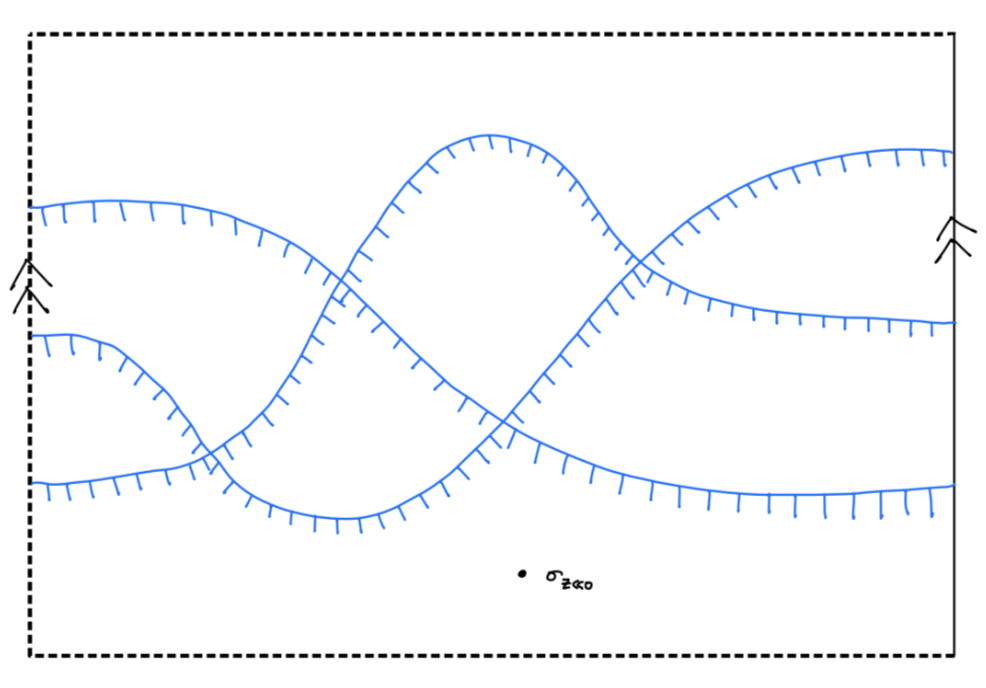
\includegraphics[scale = 0.55]{diagrams/intro/7.png}
    \caption{}
    \label{fig:your-label}
\end{figure}
Since the stratification induced by $\omega$ is not a regular cell complex, for example non-compact regions at the top and the bottom are not contractible, we refine it by adding squiggly lines co-oriented towards left.
\begin{figure}[H] 
    \centering
    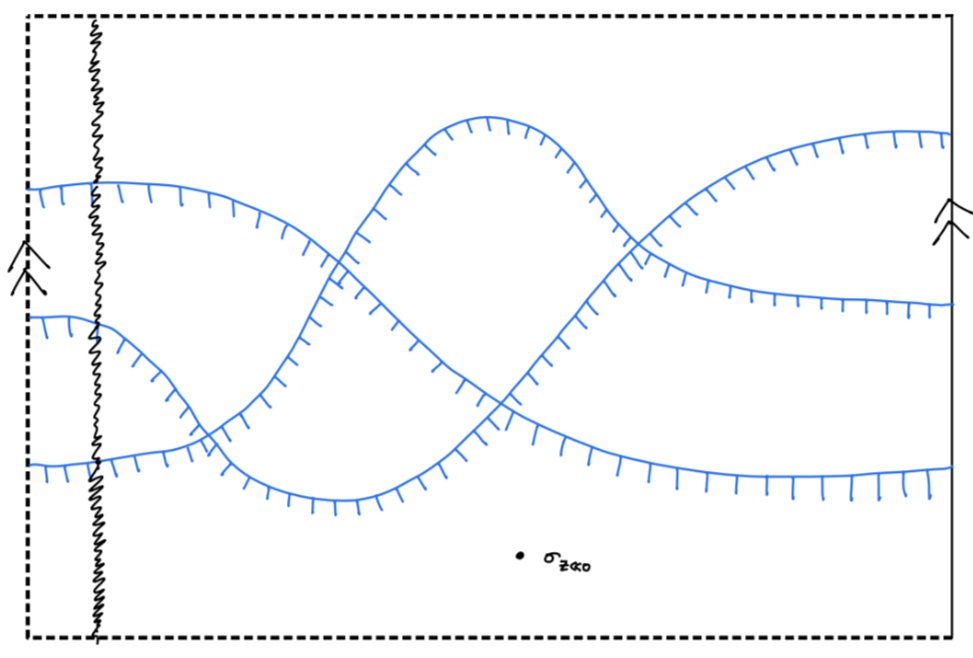
\includegraphics[scale = 0.55]{diagrams/intro/8.png}
    \caption{}
    \label{fig:your-label}
\end{figure}
Consider an object of $C_1(S^1_x \times \R_z, \Lambda_\omega, \{\sigma_{z\ll 0}\};\C)$. It can be described as a squiggly legible diagram by assigning cochain complexes of $\C$-vector spaces to regions and cochain maps to arcs subject to the conditions mentioned in (legible object subsection). Let's check how those conditions translates to our situation:
\begin{itemize}
\item the cochain complex assigned to the bottom region, which we call height $0$ region, is acyclic because of the vanishing condition at $\sigma_{z\ll 0}$. We are considering cochain complexes of sheaves upto quasi-isomorphism, so we assign $0$ stalk to the region.

\item the stalk at the regions adjacent to the height $0$ region that are not a height $0$ region, which we call height $1$ regions, should be quasi-isomorphic to dimension $1$ vector space $\C$ because of the microlocal rank $1$ condition on blue arcs separating height $0$ region and height $1$ regions i.e. the mapping cone of the cochain map corresponding to blue arcs should be rank $1$ vector spaces concentrated in degree $0$. Therefore, we assign $\C$ to these height $1$ regions and incoming maps from the height $0$ region zero maps.

\item the stalk at the regions adjacent to the height $1$ regions that are not height $0,1$ regions, which we call height $2$ regions, should be quasi-isomorphic to dimension $2$ vector space $\C^2$ and incoming maps from the height $1$ region to be monomorphisms because of the microlocal rank $1$ condition again. Therefore, we assign $\C^2$ to the height $2$ regions and incoming maps from the height $1$ regions to be inclusion maps.

\item Now, we are left with one non-compact region at the top which we call height $3$ region. Again by microlocal rank $1$ condition, the stalk should be $\C^3$ and the incoming maps from height $2$ regions are inclusion maps.

\item the maps corresponding to squiggly lines are isomorphisms of adjacent vector spaces.

\item all diagrams should commute.

\item for each crossing the crossing condition translates to
\begin{figure}[H] 
    \centering
    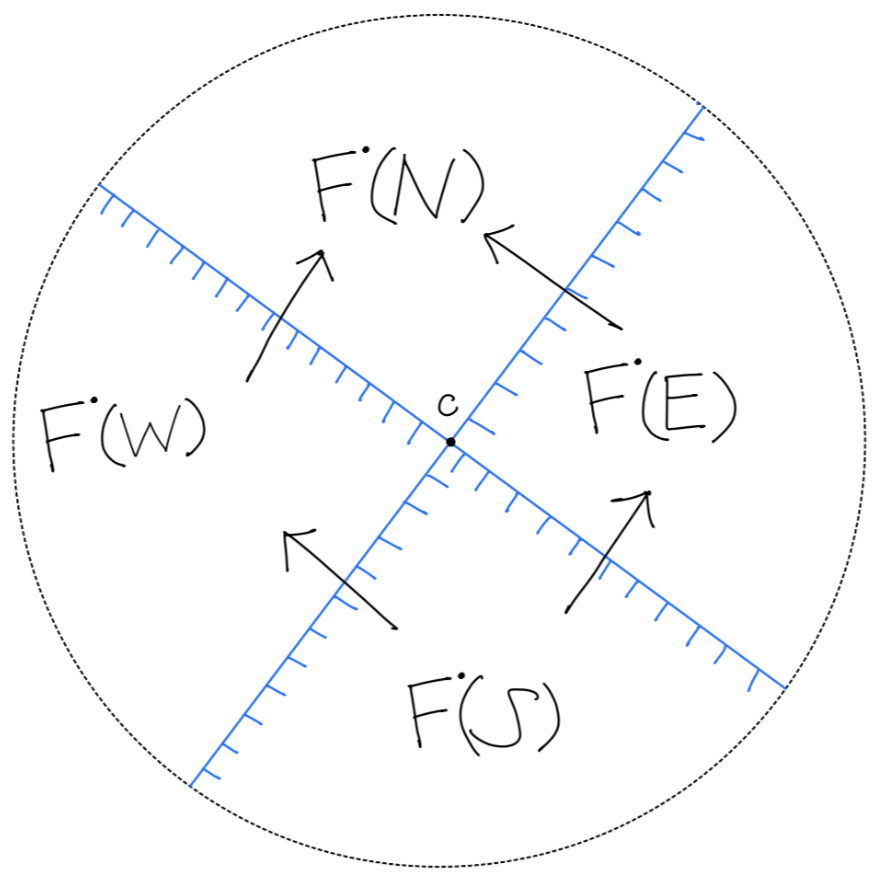
\includegraphics[scale = 0.55]{diagrams/intro/9.png}
    \caption{}
    \label{fig:your-label}
\end{figure}
\begin{figure}[H] 
    \centering
    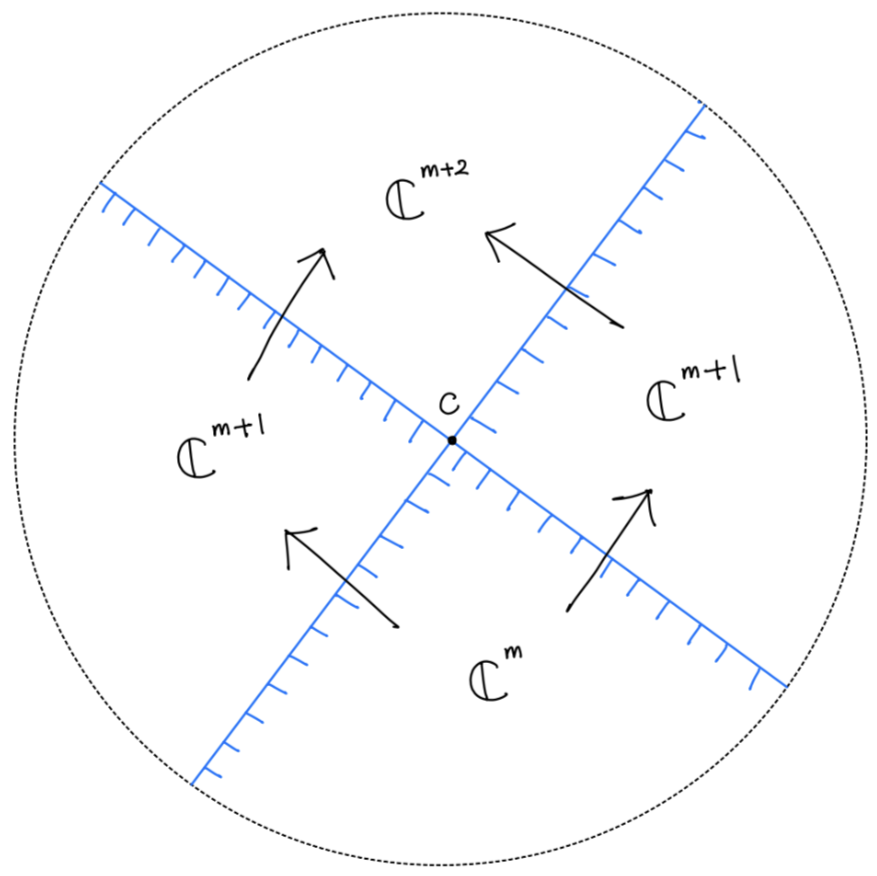
\includegraphics[scale = 0.55]{diagrams/intro/10.png}
    \caption{}
    \label{fig:your-label}
\end{figure}
the inclusion of $F^\bullet(W)$ and $F^\bullet(E)$ in $F^\bullet(N)$ intersects transversely in $F^\bullet(S)$.
\end{itemize}

In summary, an object of $C_1(S^1_x\times \R_z,\Lambda,\{\sigma_{z\ll 0}\};\C)$ amounts to the data of assigning 
\begin{itemize}
\item  dimension $i$ subspaces of $\C^3$ to height $i$ regions subject to the condition that $F^\bullet(W)+F^\bullet(E) = F^\bullet(N)$ and $F^\bullet(W)\cap F^\bullet(E) = F^\bullet(S)$.

\item an element $g \in GL_3(\C)$ that maps the subspaces corresponding to the region to the left of squiggly lines to the subspaces corresponding to the region to the right of the squiggly lines.
\end{itemize}
One thing to note in the above example is that once we assign the dimension $1$ subspaces to the height $1$ regions, all the other subspaces are determined by the crossing conditions. More precisely, we can construct subspaces that are assigned to the regions of heights greater than $1$ as follows: Suppose $R$ is a region, then the subspace we assign to $R$ is the subspace of $\C^3$ spanned by the $1$ dimensional subspaces assigned to the height $1$ regions that have paths to $R$. I will describe what this means in Chapter2. This fact that the sheaf is completely determined by its rank $1$ stalks relies on following feature of the diagram $\Lambda_\omega$:
\begin{quote}
Every region of height bigger than $1$ has more than or equal to $2$ different regions of height $1$ less adjacent to it.
\end{quote}
We call a braid word with the above property as Sibuya braid word and a braid with Sibuya braid word representation as Sibuya braid.\\
But also note that not all assignments of $1$ dimensional subspaces of $\C^3$ to height $1$ regions gives rise to legitimate sheaves. In Chapter2, I will show how to restate the crossing conditions using only rank $1$ stalks.\\
At the end of the Chapter, we will explicitly compute examples of the generalized Sibuya space.
\subsubsection*{Chapter 3}
Chapter3 is the longest chapter in the thesis, but we can summarize it more briefly:
\begin{enumerate}[label = (\roman*)]
\item we will systematically construct a natural alternating Legendrian(equivalently, alternating strand diagram) that are Legendrian isotopic to the separated Legendrian $\Lambda_\omega \coprod \Lambda_{\omega_\emptyset} \subset T^\infty(S^1_x \times \R_z)$.

\item we will construct a Legendrian isotopy between the alternating Legendrians and the separated Legendrians.

\item we will explicitly describe the sheaf cobordism induced by the above isotopy.
\end{enumerate}


\section{Conventions and notation}\label{sec_conventions}
\begin{itemize}[label={--}]
\item $\omega$ denotes positive braid words. In this thesis, all braid words are positive braid words.

\item $\beta$ denotes positive braids. In this thesis, all braids are positive braids.

\item $\operatorname{Cross}(\omega)$ denotes the set of crossings in the braid word $\omega$.

\item $L$ denotes Lagrangian surfaces in $T^*(S^1_x\times \mathbb{R}_z)$.

\item $\Lambda,\lambda$ denote Legendrian links in $T^\infty(S^1_x\times \mathbb{R}_z)$.

\item $\Xi,\xi$ denote co-orientations on Legendrian links.

\item $\Phi$ denotes front projections of Legendrian links on $S^1_x \times \mathbb{R}_z$.

\item $\mathcal{S}$ denotes refinements of the stratifications induced by front projections.

\item $\mathscr{F}^\bullet$ denotes a cochain complex of sheaves whose cohomologies are constructible sheaves. We simply call these ``sheaves" in this thesis.

\item $Q$ denotes quivers.

\item $\operatorname{Vert}(Q)$ denotes the set of vertices of the quiver $Q$.

\item $\operatorname{Arr}(Q)$ denotes the set of arrows of the quiver $Q$.

\item $\Upsilon^k_0$ denotes the set of signature $0$ height $k$ vertices in a quiver.

\item $I_k(v)$ denotes the set of height $1$ vertices that have paths to vertex $v$ in a quiver.

\item $\operatorname{SS}(\mathscr{F}^\bullet)$ denotes the singular support of the sheaf $\mathscr{F}^\bullet$.

\item $\mu mon(\mathscr{F}^\bullet)$ denotes the microlocal monodromy sheaf of $\mathscr{F}^\bullet$.

\item $Sh^\bullet(M;\mathbb{C})$ denotes the dg category of sheaves on $M$.

\item $Sh^\bullet_L(M;\mathbb{C})$ denotes the full subcategory of $Sh^\bullet(M;\mathbb{C})$ whose singular support is contained in the Lagrangian $L$.

\item $Sh^\bullet_\Lambda(M;\mathbb{C})$ denotes the full subcategory of $Sh^\bullet(M;\mathbb{C})$ whose singular support is contained in the Lagrangian $\mathbb{R}_+ \Lambda \cup 0_M$.

\item $Fun^\bullet(\mathcal{S},\mathbb{C})$ denotes the dg category of functors from the poset category $\mathcal{S}$ to the category of cochain complexes of $\mathbb{C}$-vector spaces.

\item $Fun^\bullet_\Lambda(\mathcal{S},\mathbb{C})$ denotes the full subcategory of $Fun^\bullet(\mathcal{S},\mathbb{C})$ whose objects under the quasi-equivalence $\Gamma_\mathcal{S}$ (see \ref{KS}) correspond to sheaves singular supported in $\mathbb{R}_+ \Lambda \cup 0_M$.

\item $F^\bullet$ denotes quiver representations valued in the cochain complex of $\mathbb{C}$-vector spaces.

\item $\overline{F}^\bullet$ denotes objects of $Fun^\bullet(\mathcal{S},\mathbb{C})$.

\item $\mathcal{C}_n(M,\Lambda,\{\sigma_1,\cdots,\sigma_k\};\mathbb{C})$ denotes the full subcategory of $Sh^\bullet_\Lambda(M;\mathbb{C})$ consisting of rank $n$ objects.

\item $\mathcal{M}_n(M,\Lambda,\{\sigma_1,\cdots,\sigma_k\};\mathbb{C})$ denotes the moduli space parametrizing objects of $\mathcal{C}_n(M,\Lambda,\{\sigma_1,\cdots,\sigma_k\};\mathbb{C})$.

\item $\mathcal{M}_\omega$ denotes the moduli space $\mathcal{M}_1(S^1_x \times \mathbb{R}_z,\Lambda_\omega,\{\sigma_{z\ll 0}\};\mathbb{C})$.

\item $\mathcal{M}_\omega^{fr}$ denotes the framed moduli space of $\mathcal{M}_\omega$, i.e., the moduli space parametrizing the objects of $\mathcal{M}_\omega$ with a choice of basis for the stalk at $\sigma_{z\gg 0}$, a fixed point in the non-compact region $z\gg 0$.

\item $\iota_\omega$ denotes the embedding of $\mathcal{M}_\omega^{fr}$ in the product of a general linear group with powers of projective spaces, i.e., $GL_n(\mathbb{C}) \times (\mathbb{P}^{n-1})^k$.

\item $L_{conj}$ denotes the conjugate surface of an alternating Legendrian.

\item $\Gamma_{bi}$ denotes the bipartite graph associated to an alternating Legendrian.

\item $\Psi(x_0,r_0,z_{lo},z_{hi})$ denotes the bump function about $x=x_0$ of radius $r_0$, with $z$ range from $z_{lo}$ to $z_{hi}$ i.e. consider the standard bump function 
$$\Psi_0(x) = \begin{cases}
  e^{\frac{1}{x^2 -1}}, & |x| < 1 \\
  0, & |x| \geq 1
  \end{cases}$$
then
\[
\Psi(x_0,r_0,z_{lo},z_{hi}) := (z_{hi} - z_{lo})\Psi(\frac{x-x_0}{r_0}) + z_{lo}
\]
We denote the bump function about $x=0$ of radius $1$ by $\Psi(z_{lo},z_{hi})$.

\item $\tau$ denotes the smooth transition function i.e. consider the function
  $$f(x) = \begin{cases}
  e^{-\frac{1}{x}}, & x > 0 \\
  0, & x \leq 0
  \end{cases}$$
then
  $$\tau(x) = \frac{f(x)}{f(x)+f(1-x)}$$

\item $I$ denotes an identity matrix. We omit the size of the matrix when it can be inferred from context.

\item $I_{i_0,j_0}$ denotes the matrix whose $(i,j)$-entry is $\delta_{i,i_0}\cdot \delta_{j,j_0}$ where $\delta$ is the Kronecker delta.

\item Let $T$ be an $n$ by $m$ matrix, then $T(r_{start},r_{end},c_{start},c_{end})$ denotes the truncation of the matrix $T$ with row range from $r_{start}$ to $r_{end}$ and column range from $c_{start}$ to $c_{end}$.

\item $\text{diag}(a_1,\cdots, a_k)$ denotes the diagonal matrix of size $k\times k$ whose $(i,i)$-entry is $a_i$.

\item $e_i$ denotes the $i^{\text{th}}$ standard basis vector of $\mathbb{C}^m$.

\item $\iota_k$ denotes the monomorphism from $\mathbb{C}^m$ to $\mathbb{C}^{m+1}$ that maps $e_i$ to $e_{i+k}$. We omit the dimensions of the source and the target vectorspaces when it can be inferred from the context.

\item $D_{r=r_0}$ denotes the standard disk in $\mathbb{R}^2$ of radius $r_0$ centered at the origin.

\item Let $(C^\bullet,\delta^\bullet)$ and $(C'^\bullet,\delta'^\bullet)$ be cochain complexes supported in degrees $0$ and $1$, and let $\phi^\bullet$ be a morphism between $(C^\bullet,\delta^\bullet)$ and $(C'^\bullet,\delta'^\bullet)$. Then:
\begin{itemize}[label = $\circ$]
\item We denote $(C^\bullet,\delta^\bullet)$ as either:
\begin{itemize}
\item $C^0 \xrightarrow{\delta^1} C^1$
    
    or
    
\item $\begin{array}{c}
      C^1 \\
      \uparrow^{\delta^1} \\
      C^0
      \end{array}$
\end{itemize}
\item We denote $\phi^\bullet$ as either:
\begin{itemize}
\item ($\phi^0$, $\phi^1$)
    
    or
    
\item $\begin{array}{ccc}
      C^1 & \xrightarrow{\phi^1} & C'^1 \\
      \uparrow^{\delta^1} & & \uparrow^{\delta'^1} \\
      C^0 & \xrightarrow{\phi^0} & C'^0
      \end{array}$
\end{itemize}
\item We omit coboundary maps ($\delta^1$) or cochain maps ($\phi^i$ for $i=0,1$) when either the source or the target is $0$, in which case the map is obviously a zero map.
    
\item When the source and target vector spaces of coboundary maps ($\delta^1$) or cochain maps ($\phi^i$ for $i=0,1$) are identical and the map between them is omitted, it is understood to be an identity map.

\end{itemize}
\item When drawing a squiggly legible diagram, we follow these conventions:
\begin{itemize}[label=$\circ$]
\item All maps corresponding to red arcs are $\iota_0$ unless otherwise specified.
  
\item All maps corresponding to blue arcs are $\iota_1$ unless otherwise specified.
  
\item Stalks and generization maps are omitted when they can be inferred from the context.
\end{itemize}
\end{itemize}